\documentclass[a4paper]{article}
\usepackage[
pdftex,
colorlinks=true,
bookmarksnumbered=true,
bookmarksopen=true,
bookmarksopenlevel=3,
pdfstartview=FitP,
urlcolor=blue,
]{hyperref}
\pdfinfo{
	/Title(Esercitazione di Laboratorio: Amplificatori operazionali con retroazione)
	/Author(Coa Giulio, Licastro Dario, Montano Alessandra)
}
\usepackage[italian]{babel}
\usepackage{geometry,titling,mdsymbol,stmaryrd,graphicx,subcaption,amsmath}
\graphicspath{{./Image/}}
\renewcommand\maketitlehooka{
	\null
	\mbox{}
	\vfill
}
\renewcommand\maketitlehookd{
	\vfill
	\null
}
\title{
	\begin{center}
		Esercitazione di Laboratorio:
	\end{center}
	\newline
	\begin{center}
		Amplificatori operazionali con retroazione
	\end{center}
}
\author{
	Coa Giulio
	\and
	Licastro Dario
	\and
	Montano Alessandra
}
\begin{document}
	%-----------------------------------------------------------------------------
	%  TITLE
	%-----------------------------------------------------------------------------
	\begin{titlingpage}
		\maketitle
	\end{titlingpage}
	\newpage
	%-----------------------------------------------------------------------------
	%  PURPOSE OF THE EXPERIENCE
	%-----------------------------------------------------------------------------
	\section{Scopo dell'esperienza}
	Gli scopi di questa esercitazione sono:
	\begin{itemize}
		\item Analizzare il comportamento e misurare i parametri di amplificatori reazionati.
		\item Verificare alcune deviazioni rispetto al comportamento previsto con i modelli ideali.
	\end{itemize}
	%-----------------------------------------------------------------------------
	%  INSTRUMENTATION USED
	%-----------------------------------------------------------------------------
	\section{Strumentazione utilizzata}
	La strumentazione usata durante l'esercitazione è:
	\begin{center}
		\begin{tabular}{ |c|c|c| }
			\hline
			\multirow{\textbf{Strumento}}	 & \textbf{Marca e Modello} & \textbf{Caratteristiche} \\
			\hline
			\multirow{Oscilloscopio}		 & Rigol DS1054Z			& 4 canali, \\
											 &							& $ B = 50 \, \mathrm{MHz} $, \\
											 &							& $ f_{\mathrm{c}} = 1 \, \mathrm{G\frac{Sa}{s}} $, \\
											 &							& $ R_{\mathrm{i}} = 1 \, \mathrm{M\Omega} $, \\
											 &							& $ C_{\mathrm{i}} = 13 \, \mathrm{pF} $, \\
											 &							& $ 12 \, \mathrm{Mbps} $ di profondità di memoria \\
			\multirow{Generatore di segnali} & Rigol DG1022				& 2 canali, \\
											 &							& $ f_{\mathrm{uscita}} = 20 \, \mathrm{MHz} $, \\
											 &							& $ Z_{\mathrm{uscita}} = 50 \, \mathrm{\Omega} $ \\
			\multirow{Alimentatore in DC}	 & Rigol DP832				& 3 canali \\
			\multirow{Scheda premontata}	 & A3						& \\
			\multirow{Cavi coassiali}		 &							& Capacità dell'ordine dei $ 80 \div 100 \, \mathrm{p\frac{F}{m}} $ \\
			\multirow{Connettori}			 &							& \\
			\hline
		\end{tabular}
	\end{center}
	%-----------------------------------------------------------------------------
	%  THEORETICAL PREMISES
	%-----------------------------------------------------------------------------
	\section{Premesse teoriche}
		\subsection{Incertezza sulla misura dell'oscilloscopio}
			La misura del valore di un segnale tramite l’oscilloscopio (sia esso l'ampiezza, la frequenza, il periodo, etc.) presenta un'incertezza che dipende, principalmente, da due fattori:
			\begin{itemize}
				\item l’incertezza strumentale introdotta dall’oscilloscopio (ricavabile dal manuale).
				\item l’incertezza di lettura dovuta all’errore del posizionamento dei cursori.
			\end{itemize}
			Quest’ultima incertezza deriva dal fatto che il segnale visualizzato non ha uno spessore nullo sullo schermo.
		\subsection{Amplificatore}
			Un amplificatore è un doppio bipolo unidirezionale caratterizzato dalla seguente relazione
			\begin{center}
				$ y(t) = A \cdot x(t) $
			\end{center}
			\newline
			Dove $ A $ è detto guadagno dell'amplifiatore.
			\begin{figure}[h!]
				\centering
				\begin{subfigure}{0.4\textwidth}
					\centering
					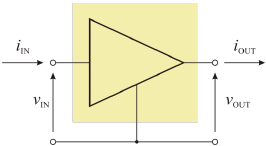
\includegraphics[scale=0.7]{amplificatore}
					\caption{Amplificatore.}
				\end{subfigure}
				\begin{subfigure}{0.4\textwidth}
					\centering
					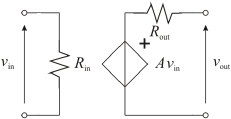
\includegraphics[scale=0.7]{amplificatoreCircuito}
					\caption{Circuito equivalente ad un amplificatore.}
				\end{subfigure}
				\label{fig:amplificatore}
			\end{figure}
			\newpage
			In base al tipo di segnale in ingresso e in uscita, possiamo distinguere quattro tipi di amplifiatori:
			\begin{itemize}
				\item Amplificatore di Tensione.
				\item Amplificatore di Transconduttanza.
				\item Amplificatore di Transresistenza.
				\item Amplificatore di Corrente.
			\end{itemize}
			\subsubsection{Amplificatore operazionale}
				L'amplificatore operazionale è un amplificatore differenziale, ovvero amplifica la differenza delle tensioni ai suoi capi, che presenta un'amplificazione $ A_{\mathrm{d}} $ idealmente infinita.
				\begin{equation*}
					\begin{split}
						A_{\mathrm{d}} &= \frac{v_{\mathrm{out}}}{v_{\mathrm{d}}} = \\
						&= \frac{v_{\mathrm{out}}}{v^{+} - v^{-}}
					\end{split}
				\end{equation*}
				\begin{figure}[h!]
					\centering
					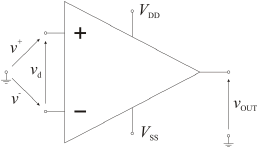
\includegraphics[scale=0.7]{amplificatoreOperazionale}
					\caption{Amplificatore operazionale}
					\label{fig:amplificatoreOperazionale}
				\end{figure}
			\subsubsection{Amplificatore differenziale}
				.
	%-----------------------------------------------------------------------------
	%  LABORATORY EXPERIENCE
	%-----------------------------------------------------------------------------
	\section{Esperienza in laboratorio}
		\subsection{Amplificatore non invertente}
			Abbiamo connesso opportunamente i coccodrilli ai nodi d'ingresso ed uscita dell'amplificatore ed alla massa, abbiamo impostato i vari interruttori nel modo richiesto.
			% calcolare il guadagno dell'amp per i 4 casi
			\newline
			Abbiamo impostato $ V_{\mathrm{pp}} = 1 \, \mathrm{V} $ e $ f = 2 \, \mathrm{kHz} $, in seguito abbiamo misurato con l'oscilloscopio $ V_{\mathrm{i}} $ e $ V_{\mathrm{o}} $.
		\subsection{Amplificatore invertente}
			.
		\subsection{Amplificatore differenziale}
			.
		\subsection{Amplificatore AC/DC}
			.
	%-----------------------------------------------------------------------------
	%  RESULTS
	%-----------------------------------------------------------------------------
	\section{Risultati}
		\subsection{Amplificatore non invertente}
			.
		\subsection{Amplificatore invertente}
			.
		\subsection{Amplificatore differenziale}
			.
		\subsection{Amplificatore AC/DC}
			.
\end{document}